\chapter{Parameter Estimation}
\label{chap:parameter-estimation}
\thispagestyle{empty}

Let us now compare the $\Lambda$CDM- and DGP-model. To do this, we will consider the ``Union2.1'' SN Ia compilation and determine best-fit values for the parameter pairs ($\Omega_{\text{m},0}$, $\Omega_{\Lambda,0}$) in $\Lambda$CDM- and ($\Omega_{\text{m},0}$, $\alpha$) in DGP-model by computing the $\chi^2$-distribution, which is a measure for the likelihood.

\section{Supernovae Type Ia ``Union2.1'' dataset}

\noindent The SN Ia ``Union2.1'' dataset (see appendix \ref{app:sn-ia-union2.1-data}) used in this thesis contains the name, the redshift, the distance modulus and the distance modulus error of 580 supernovae, measured by the Hubble Space Telescope. \\

\noindent First, let us have a look at the dataset. We plot the distance modulus (see equation \eqref{eq:distance-modulus}) $m - M$ against the redshift $z$ for the predicted luminosity distance $d_{\text{L}}$ by the $\Lambda$CDM-model with $(\Omega_{\text{m},0}, \Omega_{\Lambda,0}) = (0.3, 0.7)$ and DGP-model with $(\Omega_{\text{m}}, \alpha)=(0.3, 0.0)$.

\begin{figure}[H]
   \centering
   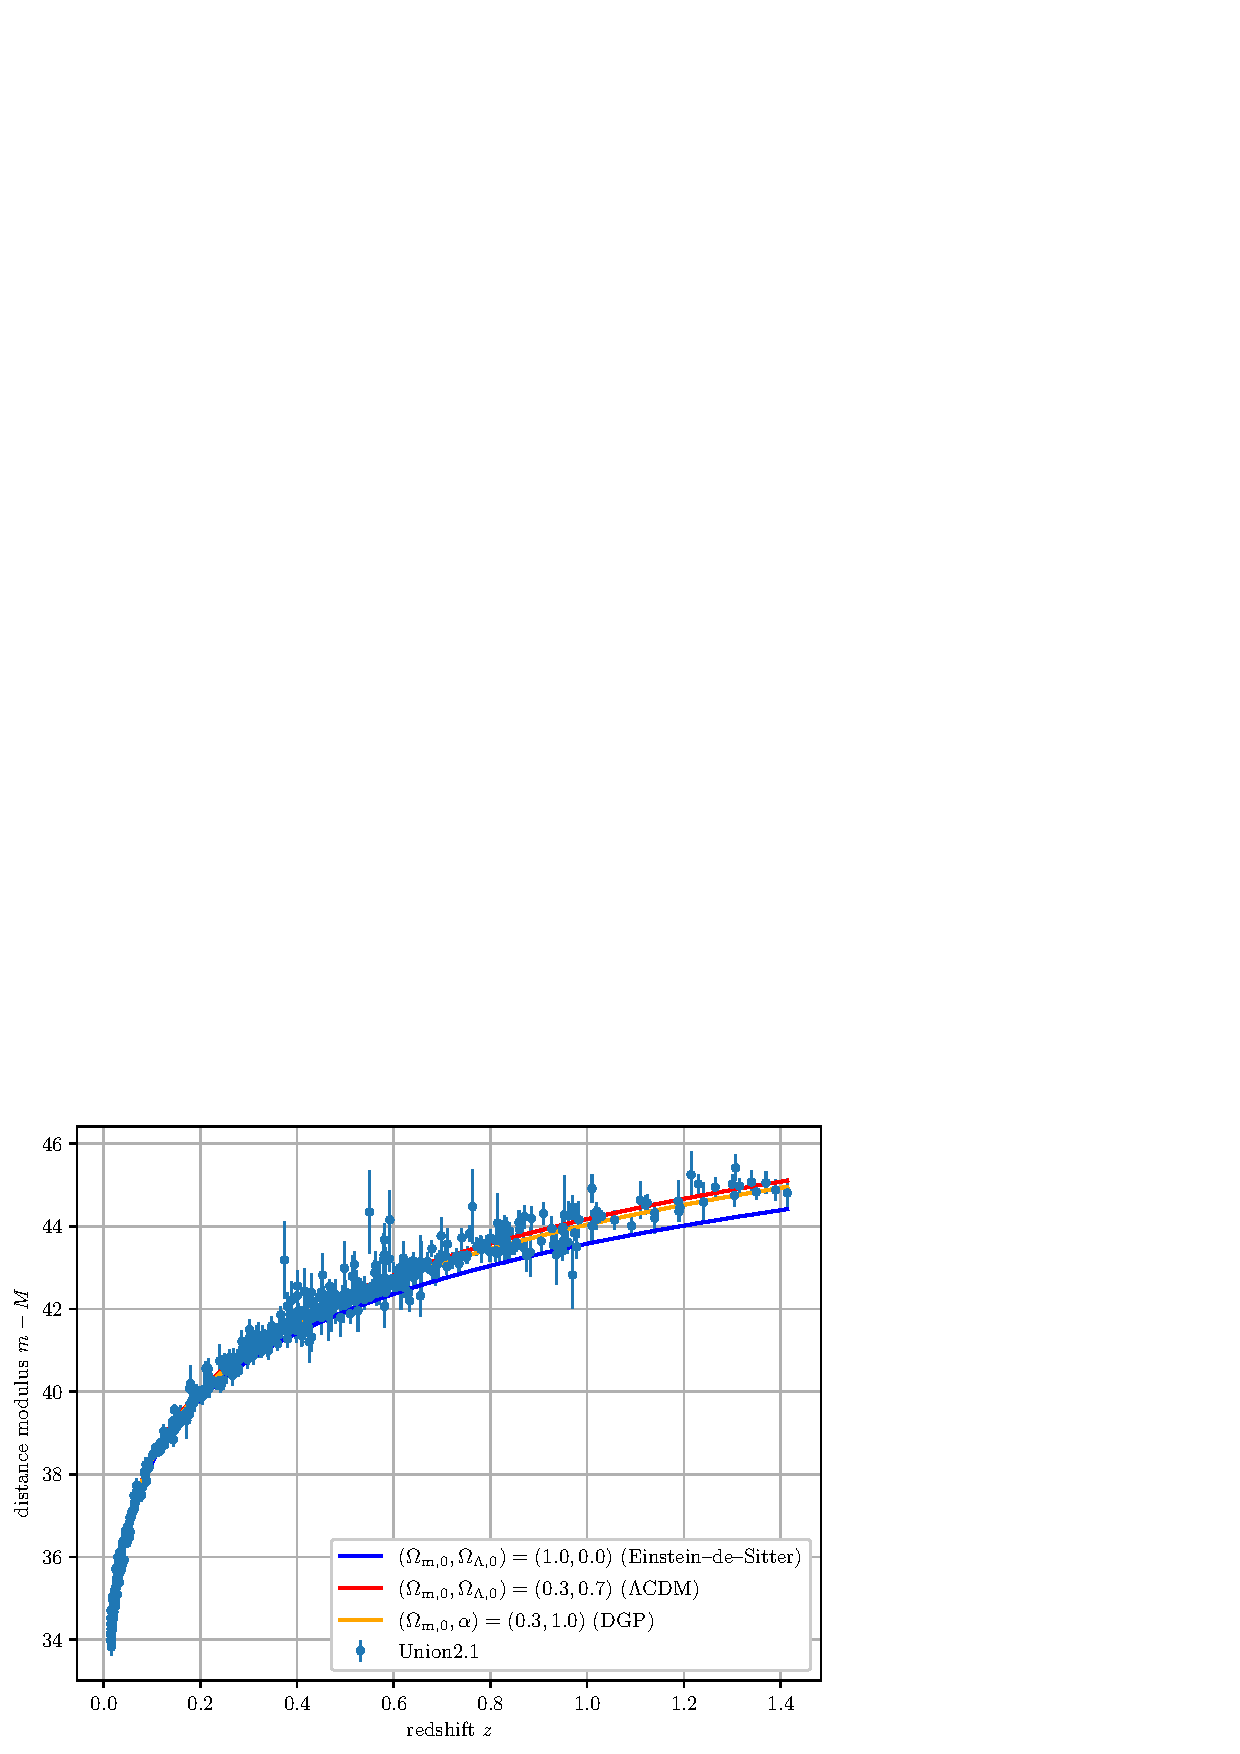
\includegraphics[scale=0.97]{figures/plots/PDF/distance-modulus_vs_redshift.pdf}
   \caption{Distance modulus $m - M$ against redshift $z$ for Einstein--de--Sitter-Model $(\Omega_{\text{m},0}, \Omega_{\Lambda,0}) = (1.0, 0.0)$, the $\Lambda$CDM-model with $(\Omega_{\text{m},0}, \Omega_{\Lambda,0}) = (0.3, 0.7)$ and DGP-model with $(\Omega_{\text{m},0}, \alpha) = (0.3, 0.0)$.\\}
   \label{fig:distance-modulus-vs-redshift}
\end{figure}

\noindent At first sight, we see that a universe that contains only matter (Einstein--de--Sitter-model) cannot match the data, especially for high redshifts. \\
Further we can conclude, that the data points at high redshift ($z \gtrsim 0.8$) have a greater influence on the fit for the estimated parameters, since there is no significant fluctuation of data points at low redshifts. \\
The apparently large errors of some data points in the range of $0.35 \leq z \leq 1.0$ should not cause any concerns whether this data set is suitable for an adequate parameter estimation, since the error of a low-redshift data point does not impact the fit that much than the error of a high-redshift data point.

\section{Statistical Analysis}
To obtain values for the best-fit parameters, we consider the distance of every data point between its measured relative magnitude to the theoretical value the relative magnitude would have dependent on the parameters of the model. \\ 
From now on, we denote $\vb*{\theta}$ as the parameter pairs of the model we want to estimate, so 
\begin{align}
    \vb*{\theta} = \begin{cases}
                        (\Omega_{\text{m},0}, \Omega_{\Lambda,0}) &\text{for $\Lambda$CDM-model}\\
                        (\Omega_{\text{m},0}, \alpha)             &\text{for DGP-model}\\
                   \end{cases}.
\end{align}
The given dataset is a sample of $N = 580$ datapoints which contain for datapoint $i \in [1,N]$ the redshift $z_{i}$, the distance modulus and therefore implicitly\footnote{Although the ``Union2.1'' SN Ia compilation contains the distance modulus $m - M$, we will handle it throughout the parameter estimation as if it only contains the relative magnitude $m$. Since we are going to marginalize the parameter $M$, it has no influence on the parameter estimation.} the relative magnitude $m_{i}$ and its error $\sigma_{m_{i}}$. \\
Our goal is to express the quantities given \textit{only} through the free parameters $\vb*{\theta}$. \\
Now, let us consider the relative magnitude $m$, which is given by the distance modulus, see equation \eqref{eq:distance-modulus}. First, we want to express the luminosity distance $d_{\text{L}}$ in multiples of $\SI{1}{\mega \parsec}$, so we obtain
\begin{align*}
    m &= M + 5\log_{10}\biggl( \frac{d_{\text{L}}}{\SI{10}{\parsec}} \biggr) = M + 5\log_{10}\biggl( 10^{5} \frac{d_{\text{L}}}{\SI{1}{\mega \parsec}} \biggr) \\
      &= M + 25 + 5\log_{10}\biggl(\frac{d_{\text{L}}}{\SI{1}{\mega \parsec}}\biggr). 
\end{align*}
Since the luminosity distance $d_{\text{L}}$ depends on the Hubble distance $d_{\text{H}}$ (see equation \eqref{eq:luminosity-distance} and \eqref{eq:comoving-distance}) and is therefore proportional to $d_{\text{L}} \propto \frac{1}{H_{0}}$, we redefine the luminosity distance so that it is independent of the Hubble constant. Hence, we go on with 
\begin{align}
m &= M + 25 + 5\log_{10} \biggl(\frac{1}{H_{0}} H_{0} d_{\text{L}}(z, H_{0}, \vb*{\theta}) \SI{}{\mega \parsec^{-1}} \biggr) \nonumber \\
  &= \underbrace{M + 25 - 5\log_{10}(H_{0})}_{ =: \mathcal{M}(H_{0}) } + 5 \log_{10} \biggl( \underbrace{H_{0} d_{\text{L}}(z, H_{0}, \vb*{\theta})}_{ =: \mathcal{D}_{\text{L}}(z, \vb*{\theta}) } \SI{}{\mega \parsec^{-1}} \biggr) \nonumber \\
  &= \mathcal{M}(H_{0}) + 5 \log_{10}(\mathcal{D}_{\text{L}}(z, \vb*{\theta}) \SI{}{\mega \parsec^{-1}}). \label{eq:relative-magnitude_new-magnitude_new-luminosity-distance}
\end{align}
With equation \eqref{eq:relative-magnitude_new-magnitude_new-luminosity-distance}, the dependency on the Hubble constant is now in an additive constant $\mathcal{M}(H_{0})$, which will be useful as we see later. \\

\noindent From now on, we are going to call the relative magnitude in equation \eqref{eq:relative-magnitude_new-magnitude_new-luminosity-distance} the \textit{theoretical} relative magnitude $m_{\text{th}}$, since it contains the cosmological parameters $\vb*{\theta}$. \\ 

\noindent For the best-fit parameter estimation, we consider the difference between the \textit{measured} value of the relative magnitude $m_{i}$ and the \textit{theoretical} value of the relative magnitude $m_{\text{th}}$. Given the dataset $D := (z_{i}, m_{i}, \sigma_{m_{i}})$, where $z_{i}$ is the measured redshift and $\sigma_{m_{i}}$ the error of the relative magnitude $m_{i}$, we define 

\begin{align}
    \chi^2(\mathcal{M}, \vb*{\theta} \vert D) := \sum_{i=1}^{N} \biggl(\frac{m_{i} - m_{\text{th}}(z_{i}, \mathcal{M}, \vb*{\theta})}{\sigma_{m_{i}}}\biggr)^2 \label{eq:chi-square} 
\end{align}
as the $\chi^2$-distribution of $\mathcal{M}$ and $\vb*{\theta}$. \\
\noindent The likelihood, which is a probability density, is given by 
\begin{align}
    L(\mathcal{M}, \vb*{\theta} \vert D) := L_{0} \exp \biggl(-\frac{1}{2} \chi^2(\mathcal{M}, \vb*{\theta} \vert D) \biggr),  \label{eq:likelihood}
\end{align}
where $L_{0}$ is a normalization factor.
With the likelihood $L$, it is possible to calculate the probability $P$ to find $\mathcal{M} \in \mathcal{I}_{\mathcal{M}}$ and $\vb*{\theta} \in \mathcal{I}_{\vb*{\theta}}$ in a parameter intervall $\mathcal{I}_{\mathcal{M}}$ and $\mathcal{I}_{\vb*{\theta}}$ with 

\begin{align}
    P(\mathcal{M} \in \mathcal{I}_{\mathcal{M}}, \vb*{\theta} \in \mathcal{I}_{\vb*{\theta}} \vert D) = \int\limits_{\mathcal{I}_{\mathcal{M}}} \dd{\mathcal{M}} \int\limits_{\mathcal{I}_{\vb*\theta}} \dd{\vb*{\theta}} L(\mathcal{M}, \vb*{\theta} \vert D). \label{eq:probability}   
\end{align}
But this probability $P$ still depends on $\mathcal{M}$, which is not measured. Since our goal is to find the best-fit values for $\vb*{\theta}$ and therefore express the probability only through $\vb*{\theta}$, we are going to \textit{marginalize} over $\mathcal{M}$. We obtain the \textit{marginalized} likelihood $\tilde{L}$ by integrating the likelihood $L$ over all possible values that $\mathcal{M}$ could take. Assuming $\mathcal{M} \in (-\infty, \infty)$, it follows  
\begin{align}
    \tilde{L}(\vb*{\theta} \vert D) = \int\limits_{-\infty}^{\infty} \dd{\mathcal{M}} L(\mathcal{M}, \vb*{\theta} \vert D). \label{eq:marginalized-likelihood} 
\end{align}
Thereby, we can calculate the probability $P(\vb*{\theta} \in \mathcal{I}_{\vb*{\theta}} \vert D)$ to find values for $\vb*{\theta} \in \mathcal{I}_{\vb*{\theta}}$, given the dataset $D$, but without any information on $\mathcal{M}$, which implicitly contains the Hubble constant $H_{0}$, so
\begin{align}
    P(\vb*{\theta} \in \mathcal{I}_{\vb*{\theta}} \vert D) = \int\limits_{\mathcal{I}_{\vb*{\theta}}} \dd{\vb*{\theta}} \tilde{L}(\vb*{\theta} \vert D). \label{eq:marginalized-probability}
\end{align}
Since $\mathcal{M}$ is only an additive constant (see equation \eqref{eq:relative-magnitude_new-magnitude_new-luminosity-distance}), this can be done analytically. We introduce the terms
\begin{align}
    c &:= \sum_{i = 1}^{N} \frac{1}{\sigma_{m_{i}}^2}, \\
    f_{0} &:= \sum_{i = 1}^{N} \frac{m_{i} - m_{\text{th}}}{\sigma_{m_{i}}^2}, \\
    f_{1} &:= \sum_{i = 1}^{N} \biggr(\frac{m_{i} - m_{\text{th}}}{\sigma_{m_{i}}} \biggl)^2
\end{align}

% \newpage 
% \begin{align*}
%     \prod_{i = 1}^{N = 2} \exp \bigl[- \alpha_{i}(x - x_{i})^2 \bigr] &= \exp \biggl[ - \bigl(\alpha_{1}(x - x_{1})^2 + \alpha_{2} (x - x_{2})^2 \bigr) \biggr] \\ 
%                                                                       &= \exp \biggl[ - \bigl( \red{\alpha_{1} x^2} - \green{2 x \alpha_{1} x_{1}} + \blue{\alpha_{1} x_{1}^2} + \red{\alpha_{2} x^2} - \green{2x \alpha_{2} x_{2}} + \blue{\alpha_{2}x_{2}^2} \bigr) \biggr] \\
%                                                                       &= \exp \biggl[ - \bigl( \red{\alpha_{1} x^2 + \alpha_{2} x^2} + \blue{\alpha_{1} x_{1}^2 + \alpha_{2} x_{2}^2} - \green{2x (\alpha_{1} x_{1} + \alpha_{2} x_{2})} \bigr) \biggr] \\
%                                                                       &= \exp \biggl[- \biggl(\sum_{i = 1}^{N = 2} \red{\alpha_{i} x^2 } + \blue{\alpha_{i} x_{i}^2} - \green{2x \sum_{i = 1}^{N = 2} \alpha_{i} x_{i}} \biggr) \biggr]
% \end{align*}



% The luminosity distance is given by  
% \begin{align}
%     d_{\text{L}}(z) = (1 + z) d_{\text{C}} = (1 + z) \frac{c}{H_{0}} \begin{cases} 
%         \frac{1}{\sqrt{\vert \Omega_{k,0} \vert}} \sin \bigl(\sqrt{\vert \Omega_{k,0} \vert} I \bigr) &\text{for} \quad \Omega_{k,0} < 0 \ (k = 1) \\
%                                                                         I &\text{for} \quad \Omega_{k,0} = 0 \ (k = 0) \\
%                                                                         \frac{1}{\sqrt{\Omega_{k,0}}} \sinh \bigl(\sqrt{\Omega_{k,0}} I \bigr) &\text{for} \quad \Omega_{k,0} > 0 \ (k = -1)
%                                                                      \end{cases}
% \end{align}
% with \eqref{eq:expansion-integral}, 
% \begin{align*}
%     I = \int\limits_{0}^{z} \dd{z'} \frac{1}{E(z')}.
% \end{align*}


% \noindent In the $\Lambda$CDM-model, the expansion function $E(z)$ contains the fit parameters $\Omega_{\text{m},0}$ and $\Omega_{\Lambda,0}$ (see \eqref{eq:expansion-function}). Since we assume that the radiation term can be neglected ($\Omega_{\text{r},0} = 0$), we obtain with \eqref{eq:density-parameters-sum}
% \begin{align}
%     \Omega_{k,0} = 1 - \Omega_{\text{m},0} - \Omega_{\Lambda,0}
% \end{align}
% and therefore 
% \begin{align}
%     E(z, \Omega_{\text{m},0}, \Omega_{\Lambda,0}) = \sqrt{\Omega_{\text{m},0}(1 + z)^{3} + \Omega_{\Lambda,0}}. 
% \end{align}

% \noindent In the DGP-model, we assume a flat universe, so $\Omega_{k,0} = 0$. We implement the polynomial equation
% \begin{align}
%     P(\Omega_{\text{m},0}, \alpha) :=  E^{2}(z) - (1 - \Omega_{\text{m},0}) E^{\alpha}(z) - \Omega_{\text{m},0} (1 + z)^{3}.
% \end{align}


\section{Computational Implementation}


\section{Results}
